\documentclass{article}

% if you need to pass options to natbib, use, e.g.:
% \PassOptionsToPackage{numbers, compress}{natbib}
% before loading nips_2018

% ready for submission
\usepackage[preprint]{nips_2018}

% to compile a preprint version, e.g., for submission to arXiv, add
% add the [preprint] option:
% \usepackage[preprint]{nips_2018}

% to compile a camera-ready version, add the [final] option, e.g.:
% \usepackage[final]{nips_2018}

% to avoid loading the natbib package, add option nonatbib:
% \usepackage[nonatbib]{nips_2018}

\usepackage[utf8]{inputenc} % allow utf-8 input
\usepackage[T1]{fontenc}    % use 8-bit T1 fonts
\usepackage{hyperref}       % hyperlinks
\usepackage{url}            % simple URL typesetting
\usepackage{booktabs}       % professional-quality tables
\usepackage{amsfonts}       % blackboard math symbols
\usepackage{nicefrac}       % compact symbols for 1/2, etc.
\usepackage{microtype}      % microtypography
\usepackage{macros}   %user custom packages

\title{Review of Papers applying Reinforcement Learning in Medical Domain}

% The \author macro works with any number of authors. There are two
% commands used to separate the names and addresses of multiple
% authors: \And and \AND.
%
% Using \And between authors leaves it to LaTeX to determine where to
% break the lines. Using \AND forces a line break at that point. So,
% if LaTeX puts 3 of 4 authors names on the first line, and the last
% on the second line, try using \AND instead of \And before the third
% author name.

\author{
  Subhojyoti Mukherjee\thanks{Use footnote for providing further
    information about author (webpage, alternative
    address)---\emph{not} for acknowledging funding agencies.} \\
  College of Information and Computer Science\\
  University of Massachusetts Amherst\\
  Massachusetts, MA 01003 \\
  \texttt{http://bio-nlp.org/index.php/people} \\
  %% examples of more authors
  %% \And
  %% Coauthor \\
  %% Affiliation \\
  %% Address \\
  %% \texttt{email} \\
  %% \AND
  %% Coauthor \\
  %% Affiliation \\
  %% Address \\
  %% \texttt{email} \\
  %% \And
  %% Coauthor \\
  %% Affiliation \\
  %% Address \\
  %% \texttt{email} \\
  %% \And
  %% Coauthor \\
  %% Affiliation \\
  %% Address \\
  %% \texttt{email} \\
}

\begin{document}
% \nipsfinalcopy is no longer used

\maketitle

%\begin{abstract}
%To be written.
%\end{abstract}

%\keywords{Changepoint, UCB1, UCB-Improved, Regret}



\section{Introduction}
\label{review:intro}
In this report we build a gadget world  for the Reinforcement Learning (RL) setup for the medical domain. A gadget problem is a simple environment which captures some of the complexities of the real-world domain which we are trying  to model. We can test various RL algorithms in this gadget worlds before transitioning to the real-world higher complexity environments. The hypothesis behind creating such gadget worlds is that if an RL algorithms performs poorly in this small gadget world, it will surely perform poorly in real-world domains.

\section{Motivational Examples}
\label{review:motivation}
We will illustrate the use of RL in medical scenarios with a few motivational examples. These will be recurring examples throughout the report. We summarize these test-cases below.

\subsection{Diabetes}

The first motivating example we state is that of treating diabetes. Diabetes is  a disease that causes a high blood glucose level in patients.
Currently there is no evident cure for this disease \citep{holt2011textbook}. There are two major sub-types of diabetes mellitus: type-1 and type-2. The treatment for diabetes consists of regulating a patient’s
blood glucose level to stay within a specific range. In order to keep their blood glucose level in an acceptable range, type-1 diabetic patients must
inject insulin several times during a day. The amount of insulin that needs to be injected depends on the amount of carbohydrate in the last meal consumed by the patient and current blood glucose level. This is because, when we eat food, our digestive system breaks the carbohydrates down to glucose. The absorption of glucose in the intestine increases its concentration in the blood stream, which puts the body into
a state of hyperglycemia (state of high blood glucose). Glucose, the key source of energy in human body, needs insulin for its routine disposal into cells. In a healthy individual, the pancreas produces
insulin, which allows muscle and fat cells to absorb glucose from blood stream. Consequently the blood glucose level decreases back to the normal level. Other mechanisms operate when the blood glucose goes below its normal value – that is, when the body enters a state of hypoglycemia. The global situation of diabetes afflicting people is shown in Figure \ref{Fig:Diabetes-IDF}.


\begin{figure}[!th]
\center
\begin{tabular}{cc}
\subfigure[2.75\textwidth][Diabetes Scenario Worldwide] 
    %with $r_{i_{{i}\neq {*}}}=0.07$ and $r^{*}=0.1$
    {
\includegraphics[scale=0.3]{img/diabetes_idf.png}
%\caption{Diabetes Scenario Worldwide}
\label{Fig:Diabetes-IDF}
}
&
\subfigure[2.75\textwidth][Sepsis severity resulting in death] 
    %with $r_{i_{{i}\neq {*}}}=0.07$ and $r^{*}=0.1$
    {
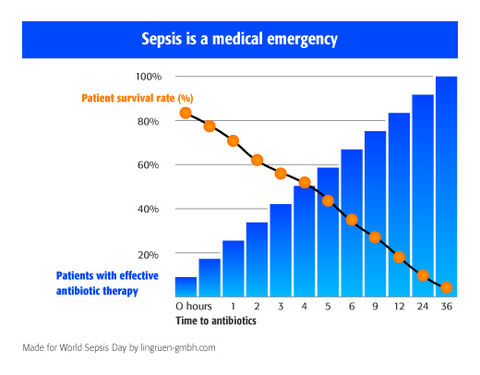
\includegraphics[scale=0.3]{img/sepsis-antibiotics.jpg}
%\caption{Sepsis severity resulting in death}
\label{Fig:Sepsis-Antibiotics}
}
\end{tabular}
\caption{Severity of Diabetes and Sepsis}
\end{figure}

\subsection{Sepsis}

Our second motivating example is sepsis treatment in ICU. Sepsis is a complication of an infection resulting out of an extreme immune system response triggering widespread inflammation throughout the body. Sepsis can range from mild to severe and because it can be potentially life-threatening, it requires sustained and immediate medical attention. Sepsis treatment varies and depends on the cause of the infection that led to sepsis, as well as the severity of symptoms. Because mild sepsis can rapidly progress to severe sepsis and then septic shock, doctors must work quickly to reduce inflammation. Common treatments for sepsis include: 1. administering Antibiotics 2. injecting Intravenous (IV) Fluids and 3. in the extreme cases when blood pressure has fallen dangerously low using Vasopressors. An illustrative figure showing the severity of sepsis leading to death resulting from delay in administering antibiotics is shown in Figure \ref{Fig:Sepsis-Antibiotics}.

%\begin{figure}[!th]
%\center
%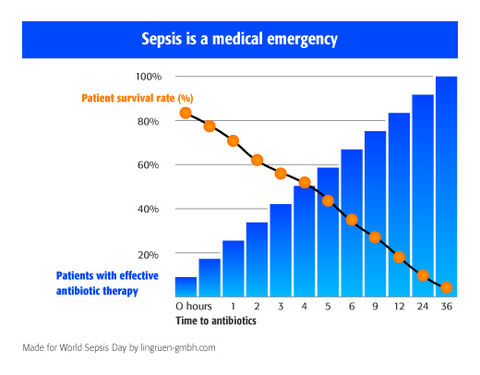
\includegraphics[scale=0.4]{img/sepsis-antibiotics.jpg}
%\caption{Sepsis severity resulting in death}
%\label{Fig:Sepsis-Antibiotics}
%\end{figure}

\section{Why Reinforcement Learning?}
\label{review:whyRL}
A large number of problems in science and engineering, robotics and game playing, resource management, financial portfolio management, medical treatment design, ad placement, website optimization and packet routing can be modeled as sequential decision-making under uncertainty. Many of these real-world interesting
sequential decision-making problems can be formulated as reinforcement learning (RL) problems (see \citep{bertsekas1996neuro}, \citep{sutton1998reinforcement}). In an RL problem, an agent interacts with a dynamic, stochastic, and unknown environment, with the goal of finding an action-selection strategy or policy that optimizes some long-term performance measure. Every time when the agent interacts with the environment it receives a signal/reward from the environment based on which it modifies its policy. The agent learns to optimize the choice of actions over several time steps which is learned from the sequences of data that it receives from the environment. This is the crux of online sequential learning. 

    This is in contrast to supervised learning methods that deal with labeled data which are independently and identically distributed (i.i.d.) samples from the considered domain and train some classifier on the entire training dataset to learn the pattern of this distribution to predict the labels of future samples (test dataset) with the assumption that it is sampled from the same domain. In contrast to this, an RL agent learns from the samples that are collected from the trajectories generated by its sequential interaction with the system. For an RL agent, the trajectory consists of a series of sequential interactions whereby it transitions from one state to another following some dynamics intrinsic to the environment while collecting the reward till some stopping condition is reached. This is known as an episode. Here, for an action $a_t$ taken by the agent at the $t$-th timestep, the agent transitions from its current state denoted by $S_{t}$ to state $S_{t+1}$ and observes the reward $R(s_t,a_t)$. An illustrative image depicting the reinforcement learning scenario is shown in Figure \ref{fig:rl}.
    

\begin{figure}[!th]
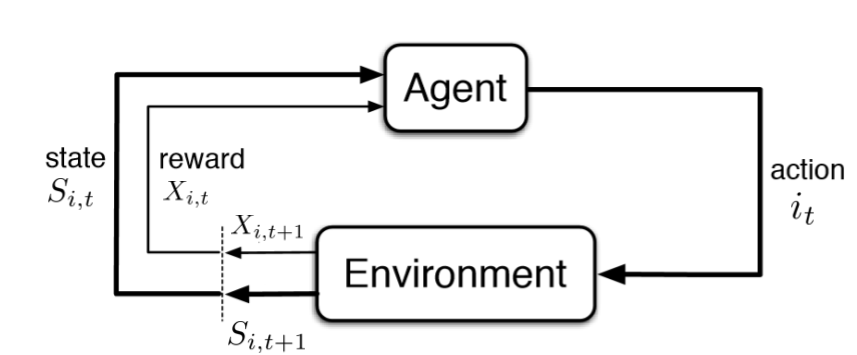
\includegraphics[scale=0.4]{img/RL1.png}
\caption{Reinforcement Learning}
\label{fig:rl}
\end{figure}

In the healthcare domain, there exists many scenarios in which the treatment involves taking a series of decisions over a long time. After every medical decision is made, and a treatment administered the condition of the patient changes. Based on this new condition of the patient medical practitioners may alter their evaluation policy to administer a new set of treatments or may continue with the last policy with the same dosage. Notice, that this is quite similar to the general RL framework where the condition of the patient can be defined by the state $S_t$, the treatment administered can be defined by action $a_t$ and after administering the treatment the new condition that the patient transitions to can be defined by $S_{t+1}$. We will formalize this setting in Section \ref{review:mdp} while we will illustrate several challenges where this simple framework will fail in real world scenarios in Section \ref{review:complexity}.

	As mentioned in \citet{DBLP:conf/embc/NematiGC16} RL is particularly well-suited for the medication dosing problem given the sequential nature of clinical treatment where multiple treatment decision are performed without immediate knowledge of effectiveness. Indeed, the lack of a one-to-one correspondence between actions and outcomes makes it difficult to assign credit or blame to individual actions along the way to an intermediate or terminal outcome. Moreover, the effect of interventions for a given patient can be non-deterministic, and attempting to predict the effects of a series of treatments over time only causes more uncertainty.



%\section{Some challenges of Medical Domain}
%\label{review:challenges}
%\input{challenges}


\section{Notations, Assumptions and Definitions}
\label{review:notations}
We use capitalized calligraphic notations to denote sets while individual elements within the set is denoted by non-capitalized alphabets. The random variables are denoted by capitalized, non-calligraphic alphabets. $\A$ denotes the finite set of actions  with individual action indexed by $A_t = a$ such that action taken at time $t$ is $a$. We assume that the total number of actions is constant throughout the time horizon. We assume that the transition function is stationary that is, it is not changing between episodes.

%$T$ denotes the time horizon. We use capitalized calligraphic notations to denote sets while individual elements within the set is denoted by non-capitalized alphabets. $\A$ denotes the finite set of actions  with individual action indexed by $a$ such that $a=1,\ldots, K$. We assume that the total number of actions is discrete and constant throughout the time horizon and $|\A|=K$. In the gridworld setting $K=4$. We define an MDP $M$ with the tuple $M  = (\S,\A,P,d_R, d_0,\gamma)$ where $\S$ is the set of states, $\A$ is the set of actions, $P$ is the transition function, $d_R$ is the reward distribution over the states indicating how the rewards are generated, $d_0$ is the initial state distribution and $\gamma$ is the discounting factor.


\section{MDP Formulation}
\label{review:mdp}


A RL setting is usually characterized by a MDP or Markov Decision Process. A MDP is defined by the tuple $\lbrace \S,\A, P, d_R, d_{0},\gamma\rbrace$ where each element of the tuple is defined as:-
\begin{enumerate}
\item $\S$ is the finite state space such that at each time step $t$ the patient is in state $S_t \in \S$. This state space can be discrete or continuous depending on the modeling assumption of the learner.
\item $\A$ is the action space such that at each time t, the agent takes
action $\A_t \in \A$, which causes it to change its state from $S_t$ to $S_{t+1}$. Again this action space can be discrete or continuous depending on the modeling assumption of the learner.
\item $P$ is the transition function which describes how the state of the environment changes. So, $P(s,a,s') = Pr(S_{t+1}=s' | S_{t} = s, A_{t} = a)$
\item $d_R$ denotes the process of reward generation when the state of the agent changes.
\item $d_0$ denotes the initial state distribution of the agent.
\item The discount factor, $\gamma$, determines the relative weight of immediate and long-term rewards. 
\end{enumerate}

The goal of the RL agent is to learn a policy, i.e. a mapping $\pi : \S \times \A \rightarrow [0,1]$  from states to actions, that maximizes the expected discounted return $G_t$

\begin{align*}
J(\pi) &= \mathbb{E}[\sum_{t=0}^{\infty}G_t | \pi] = \mathbb{E}[\sum_{t=0}^{\infty}\gamma^t R_t | \pi]
\end{align*}

where $R_t$ is all the accumulated rewards by the agent and $T$ denotes the time horizon. 

%$T$ denotes the time horizon. We use capitalized calligraphic notations to denote sets while individual elements within the set is denoted by non-capitalized alphabets. $\A$ denotes the finite set of actions  with individual action indexed by $a$ such that $a=1,\ldots, K$. We assume that the total number of actions is constant throughout the time horizon and $|\A|=K$. The state of an 


\section{Some Challenges of Medical Domain}
\label{review:complexity}
Some of the difficult features that constitute the medical domain which we try to model in this gadget world are :-

\begin{itemize}
\item The medical environment is a partially observed environment. At any instant the physician is only exposed to some of the factors influencing the health of the patient.
\item Long horizon problem where you only receive the feedback at the end of the episode or the feedbacks are very sparse in nature.
\item Time constrained treatment, which requires that the effective treatment needs to be delivered within a fixed time otherwise it may result in death.
\item Time varying adversarial feedbacks, which may be encountered in sudden spikes in responses from the patient to the treatments administered.
\end{itemize}

\section{Discussion on Algorithms}
\label{review:algorithm}
In the off-policy setting, there are two stationary Markov policies, one used
to generate the data, called the behavior policy and another one called the target policy whose value function we seek to estimate. The two policies can be completely arbitrary but subject to some constraints. The behavior policy must be soft, that is it must
have a non-zero probability of selecting every action in
each state. Some algorithms require even weaker constraints on the behavior policy that it can be stationary and non-starving. 

Off-policy evaluation is difficult because there is a mismatch of distributions. Since the learner has to estimate the target policy but is only goven samples from the behavior policy. A classical way of handling such situations comes from \citet{DBLP:books/lib/Rubinstein81} by the way of \textit{Importance Sampling}. Several interesting algorithms in the Reinforcement Learning setting have been proposed for off-policy evaluation incorporating Importance Sampling. These Per-Decision Importance Sampling \citep{DBLP:conf/icml/PrecupSS00}, Per-Decision Weighted Importance Sampling \citep{DBLP:conf/icml/PrecupSS00}, Doubly Robust Importance \citep{DBLP:journals/corr/JiangL15} Sampling and Weighted Doubly Robust Importance Sampling \citep{DBLP:conf/icml/ThomasB16}. 

Fitted Q iteration (FQI) is a batch RL algorithm whose main fea-
ture lies in the way that it handles the experience \citep{DBLP:journals/jmlr/ErnstGW05}. Unlike incremental algorithms like Watkin's Q-learning \citep{DBLP:journals/ml/WatkinsD92}, FQI uses the complete set of transitions each time that updates the estimation of the optimal Q-function. Although this process involves more computation, it allows to extract more information from the stored experience. Conse-
quently, FQI is more data-efficient than other RL algorithms. This feature makes FQI a very suitable algorithm in many application domains. In certain scenarios it is quite expensive to conduct an experiment with respect to both money and time. For, example administering a dose to a patient and waiting to observe its effect. Thus, reducing the quantity of data required by the algorithm can be crucial.


\section{Related Papers}
\label{review}
We first review the papers related to sepsis, ICU patients, Lung Cancer, Epilepsy, Heparin Dosing treatment.

\begin{table}[!th]
%\begin{center}
%\vspace*{-1.5em}
\caption{Review of papers}
\label{tab:review1}
\begin{tabular}{|p{3 em}|p{3 em}|p{3 em}|p{3em}|p{6em}|p{10em}|p{5 em}|p{6em}|}
\toprule
Paper  & Disease  & Algo type & MDP info & Contributions  & Approach & Conclusions/ Observations  & Limitations \& Future Works \\
\hline
\citet{DBLP:journals/corr/RaghuKCSG17} & Sepsis 
& 
Dueling Double-Deep Q Network (Off-policy algorithm)
& 
\textbf{1)} Continuous States
\textbf{2)} Discrete Actions
&  
\textbf{1)} Deep RL models with continuous-state spaces, improving on earlier work with discretized models.
\textbf{2)} Identify treatment policies that could improve patient outcomes
\textbf{3)} Investigate the learned policies for clinical interpretability
&
\textbf{1)}  Q-values are frequently overestimated in practice,
leading to incorrect predictions and poor policies. So, uses Double-Deep Q Network, where the target Q values are determined using actions found through a feed-forward pass on the main network, as opposed to being determined directly from the target network. \textbf{2)} For finding optimal treatments, they separate the influence on Q-values of a) a patient’s underlying state being good (e.g. near discharge), and b) the correct action being taken at that timestep. So, uses a Dueling Q Network, where the action-value function for a given (s, a) pair, Q(s, a), is split into separate value and advantage streams. The value stream represents the quality of the current state, and the advantage represents the quality of the chosen action. Training such a model can be slow as reward signals are sparse and only available on terminal timesteps. They use Prioritized Experience Replay to accelerate learning by sampling a transition from the training set with probability proportional to the previous error observed.
& 
Their policies learned that vasopressors may
not be a good first response to sepsis and maybe harmful in some populations.
& 
\textbf{1)} The reward assignment in this model is quite sparse, with rewards/penalties only being issued at terminal states. There is scope for improvement here; one idea could be to use a clinically informed reward function based on patient blood counts to help learn better policies. \textbf{2)} Another approach could be to use inverse RL techniques to derive a suitable reward function based on the actions of experts (the physicians). 
   \\\midrule
\end{tabular}
\vspace*{-2em}
%\end{tabular}
%\end{center}
\end{table}   



\begin{table}[!th]
%\begin{center}
%\vspace*{-1.5em}
\caption{Review of papers}
\label{tab:review2}
\begin{tabular}{|p{3 em}|p{3 em}|p{3 em}|p{3em}|p{6em}|p{10em}|p{5 em}|p{6em}|}
\toprule
Paper  & Disease  & Algo type & MDP info & Contributions  & Approach & Conclusions/ Observations  & Limitations \& Future Works \\
\hline
\citet{DBLP:journals/corr/abs-1712-00654} & Sepsis 
& 
Off-policy evaluation using policy iteration for $\pi^*$, $\pi^r$ from real trajectories.
& 
\textbf{1)} Discrete State Space, with patient conditions being noted at regular intervals.
\textbf{2)} Discrete Actions with continuous glucose level being categorized into 11 bins.
&  
\textbf{1} They hypothesize that the patient states, glycemic values, and patient outcomes can be modeled by a Markov decision process (MDP) whose parameters and optimal policies can be learned from data. \textbf{2)} They develop a decision support for glycemic control to target specific ranges of serum glucose that optimizes outcomes and is  personalized for each patient depending on their specific circumstances.
%optimize outcomes for patients personalized for each patient depending on their specific circumstances.
%
%They do not recommend specific interventions such as insulin oral hypoglycemic agent administration to achieve the target goals, but focus on finding the optimal targets. Thus the action  formulation is choosing the best glycemic target under the circumstances of the patient at that time. They  leaving the choice of agents and doses to achieve that target to the clinicians. This simplification avoids the need to model the variability of patients’ glycemic responses to actual insulin doses and avoids data problems with incorrectly recorded dose timing.
&
\textbf{1)} To learn the patient state representation they use two types of
feature representations: raw interpretable clinical features and the feature representation generated
by a sparse autoencoder. After they generate the state representation, they categorize the patients into 500 clusters by using k-means clustering algorithm. \textbf{2} Policy Iteration algorithm is used to learn $\pi^*$ which is the behavior policy. The estimation policy $\pi^r$ is evaluated based on real trajectories where they  limited the action space of each state to only the one with the highest probability in the transition matrix  instead of exploring all possible actions. \textbf{3)} $\pi^r$ and real mortality rate were used
to obtain the estimated \textit{mortality–expected return function}, which reveals the relationship between
expected return and the estimated 90-day mortality rate. This function was used to compute and
compare the estimated mortality rate of real and optimal glycemic trajectories obtain by $\pi^r$ and $\pi^*$
& 
\textbf{1)} If clinicians chosen dosages can actually achieve the target glucose
levels chosen by the policy then it may reduce the
mortality rate of septic patients. \textbf{2)} Their mortality–expected return function shows that using raw feature representation or learned feature representation using autoencoder may yield a good result, that is both are close to mortality rate calculated from the real data.
%result indicate that the learned expected return reflects the real patient status well. They compute the empirically estimated mortality rate of the real glycemic trajectory using the mortality–expected return function acquired from raw and encoded patient state representations. The average expected 90-day mortality rate of the testing
%dataset is 31.00\% using the raw feature representation, and 31.08\% using the sparse autoencoder
latent representation. Both are close to the mortality rate calculated from the real data (31.17\%).
& 
\textbf{1)} State space is discrete, which is an issue. \textbf{2)} The off policy evaluation needs to be better.
   \\\midrule
\end{tabular}
\vspace*{-2em}
%\end{tabular}
%\end{center}
\end{table}   


\begin{table}[!th]
%\begin{center}
%\vspace*{-1.5em}
\caption{Review of papers}
\label{tab:review3}
\begin{tabular}{|p{3 em}|p{3 em}|p{3 em}|p{3em}|p{6em}|p{8em}|p{7 em}|p{6em}|}
\toprule
Paper  & Disease  & Algo type & MDP info & Contributions  & Approach & Conclusions/ Observations  & Limitations \& Future Works \\
\hline
\citet{DBLP:journals/corr/abs-1805-12298}  \textbf{This paper is very impt. as it is like a review paper detailing the challenges}& Sepsis 
& 
Comapre Per-Decision Importance Sampling (PDIS), Weighted Per-decision Importance sampling (WPDIS), Doubly-Robust (DR), and Weighted Doubly-Robust (WDR).
& 
\textbf{1)} Discrete State Space, with patient conditions being noted at regular intervals.
\textbf{2)} Discretized treatment IV fluids and vasopressors each into 5 bins, the first representing
no treatment (zero dosage), and the rest representing quartiles of the actions prescribed by
physicians. Hence total 25 actions.
\textbf{3} Reward is zero till the last action.
&  
\textbf{1)} Data needs to be processed correctly otherwise the susceptibility of AI algorithms to learn harmful policies due to artifacts in the data increases. \textbf{2)} The algorithm learns to recognize patients who need additional care \textit{but} lack of options in actions makes the algorithm choose intubation which is not recommended. \textbf{3)} They observed the learned policies recommend minimal treatment for patients with very high SOFA (Sequential Organ Failure Assessment) score. This recommendation is faulty but algorithms predict this because the mortality rate for this subpopulation is high and hence the policy have not learnt what to do.
&
\textbf{1)} The weighted methods (WPDIS, WDR) trade increased bias for reduced variance, while the per decision methods reduce variance by computing the weights in a way that does not
penalize the probability of a current action based on future ones. \textbf{2)} Doubly robust methods (DR, WDR) leverage an approximate model of the reward function to reduce variance. \textbf{3)} All of the policies have relatively close median values and large variances, making it hard to draw definitive conclusions. The model-based WDR estimator uses a model to reduce variance, but also inherits the optimistic bias of the model. The model-free WPDIS estimator also suffers from large variances. \textbf{4)} To the patients belonging to a lower risk group, the WPDIS method suffers from a selection bias. It predicts a no-treatment policy to these group as they have lower mortality rate.
& 
\textbf{1)}  State representation need to account for any variables that might confound estimates of outcomes under the policy. \textbf{2)} It's impossible to account for the entire history of the patient and determine/avoid such confounding variables.  Instead, domain knowledge by an expert/clinical researcher must be applied to take care of this. This is especially a difficult problem to solve in sequential setting.
& 
\textbf{1)} If outcomes are sparse then performance suffers. \textbf{2)} High variance in the performance of Importance sampling algorithms as some actions which are never tested has close to zero probability. \textbf{3)} Sufficient confidence on the action by the policies cannot be guaranteed.
   \\\midrule
\end{tabular}
\vspace*{-2em}
%\end{tabular}
%\end{center}
\end{table}   



\begin{table}[!th]
%\begin{center}
%\vspace*{-1.5em}
\caption{Review of papers}
\label{tab:review4}
\begin{tabular}{|p{3 em}|p{3 em}|p{3 em}|p{3em}|p{6em}|p{8em}|p{7 em}|p{6em}|}
\toprule
Paper  & Disease  & Algo type & MDP info & Contributions  & Approach & Conclusions/ Observations  & Limitations \& Future Works \\
\hline
\citet{DBLP:journals/corr/abs-1807-01066} & Sepsis 
& 
Per Horizon Weighted Importance sampling (PHWIS), and Per Horizon Weighted Doubly-Robust (PHWDR).
& 
\textbf{1)} Continuous State Space (Toy domain)
\textbf{2)} Discrete Action Space (Toy Domain)
&  
\textbf{1)} This work evaluates the sensitivity of off-policy evaluation
to calibration errors in the learned behaviour policy. They show how powerful parametric models such as neural networks can result in highly uncalibrated behaviour policy models on a real-world medical dataset
&
\textbf{1)} They use PHWIS and PHWDR instead of step-wise IS and DR to reduce variance. \textbf{2)} To split the horizon for estimation and behavior policy, two methods are considered, random and intervention splitting. Random splitting randomly chooses half the trajectories for each policies, while intervention splitting splits patients who have been treated with vasopressors (or not).  \textbf{3)} To compare between $\pi_e$ and $\pi_b$ the use Mean square estimation.
& 
\textbf{1)} Uncalibrated behaviour policy models can result in
highly inaccurate OPE in a simple, controlled navigation
domain.
\textbf{2)} In a real-world sepsis management domain, powerful
parametric models such as deep neural networks produce
highly uncalibrated probability estimates. Neural networks can produce overconfident and incorrect probability estimates of actions.
\textbf{3)} A simple, non-parametric, k-nearest neighbours model
is shown to be better calibrated than all the other parametric models
in their medical domain, and using this as a behaviour
policy model results in superior OPE.
& 
\textbf{1)} The proposed
procedure can be used in other situations where the
behaviour policy is unknown, and could improve the quality
of OPE estimates.
   \\\midrule
\end{tabular}
\vspace*{-2em}
%\end{tabular}
%\end{center}
\end{table}   


\begin{table}[!th]
%\begin{center}
%\vspace*{-1.5em}
\caption{Review of papers}
\label{tab:review5}
\begin{tabular}{|p{3 em}|p{3 em}|p{3 em}|p{3em}|p{6em}|p{6em}|p{6 em}|p{9em}|}
\toprule
Paper  & Disease  & Algo type & MDP info & Contributions  & Approach & Conclusions/ Observations  & Limitations \& Future Works \\
\hline
\citet{DBLP:journals/corr/PrasadCCDE17} & ICU patient 
& 
Fitted Q-Iteration wither Extra Trees and Neural Network as function  approximators .
& 
\textbf{1)} Continuous State Space 
\textbf{2)} Discrete Action Space 
\textbf{3)} They do not consider this as a POMDP
&  
\textbf{1)} This work develops a decision support tool to alert clinicians when a patient is ready for weaning (taken off mechanical ventilation). \textbf{2)} It uses available patient information in the 
ICU setting and proposes the off-policy Fitted Q-Iteration (FQI) algorithm with different regressors for optimal treatment.
&
\textbf{1)} Simple Q-Learning using 3 layers of hidden layer fails to learn propoerly. \textbf{2)} They use FQI (with batch mode learning) with Regressor as Extra Trees for Function approximation and this performs well. \textbf{3)} Neural FQI with 3 hidden layers for function approximation also performs well in this dataset. Neural FQI achieves a four-fold gain in performance as compared to FQI with extra trees. 
& 
\textbf{1)} They show that the algorithm
is capable of extracting meaningful indicators in recommending extubation time and sedation levels, on average outperforming clinical
practice in terms of regulation of vitals and reintubations for patients.
& 
\textbf{1)} Policies must show some invariance to reward shaping. The current methods display considerable sensitivity to the relative weighting
of various components of the feedback received after each
transition. A more principled approach to the design of the reward function, for example by applying techniques in inverse
reinforcement learning \citep{DBLP:conf/icml/NgR00}, can help
tackle this sensitivity. 
\textbf{2)} Effective communication of the best action,
expected reward, and the associated uncertainty, calls
for a probabilistic approach to estimation of the Q-function,
which can perhaps be addressed by pairing regressors such
as Gaussian processes with Fitted Q-iteration.
\textbf{3)} Increase the sophistication of the state space by handling
long term effects more explicitly using second-order
statistics of vitals \textbf{4)} Modeling the system as a partially observable MDP, in which observations map to some underlying state
space. \textbf{5)} Extending the discrete action space to continuous action space so that continuous
dosages of specific drug types and settings such as ventilator
modes can be taken into account. 
   \\\midrule
\end{tabular}
\vspace*{-2em}
%\end{tabular}
%\end{center}
\end{table}   


\begin{table}[!th]
%\begin{center}
%\vspace*{-1.5em}
\caption{Review of papers}
\label{tab:review6}
\begin{tabular}{|p{5 em}|p{4 em}|p{3 em}|p{3em}|p{6em}|p{6em}|p{6 em}|p{6em}|}
\toprule
Paper  & Disease  & Algo type & MDP info & Contributions  & Approach & Conclusions/ Observations  & Limitations \& Future Works \\
\hline
\citet{DBLP:conf/adprl/PadmanabhanMH14} & Anesthesia of ICU patient with respiratory  disease symdromes
& 
Modified Watkin's Q-learning (on-policy).
& 
\textbf{1)} Discrete State Space 
\textbf{2)} Discrete Action Space 
&  
\textbf{1)} This work develop a RL-based closed-
loop anesthesia controller using the bispectral index (BIS) as a control variable while concurrently accounting for mean
arterial pressure (MAP). \textbf{2)} This work uses these two parameters to control propofol infusion rates to
regulate the BIS and MAP within a desired range. 
&
\textbf{1)} The states of the system
should be observable for decision making. \textbf{2)} The states of the  system are based on the measurable parameters BIS and MAP. \textbf{3)} The error is measured based on  a weighted combination of the error of the BIS(error) and MAP(error). This reduces the computational complexity of the RL algorithm and
consequently the controller processing time\textbf{4)} Finally Q-Learning is used to learn the sequence of infusion rates that results in a minimum BIS(error) and MAP(error). 
& 
\textbf{1)} In this paper, a reinforcement learning-based approach
for the simultaneous control of sedation and hemodynamic
parameter management is proposed using the regulation of
the anesthetic drug propofol. 
\textbf{2)} Simulation results using 30 patient models with varying pharmacokinetic and pharma-codynamic parameters show that the proposed RL control strategy is promising in designing closed-loop controllers for ICU sedation to regulate sedation and hemodynamic pa-
rameters simultaneously. \textbf{3)} The simulations show
that the RL-based, closed-loop control is robust to system
uncertainties. 
& 
\textbf{1)}  Discrete State and Action Space is a drawback
\textbf{2)} Too less number of patients in the experiment, so doubtful conclusions can be drawn.
   \\\midrule
\end{tabular}
\vspace*{-2em}
%\end{tabular}
%\end{center}
\end{table}   

\begin{table}[!th]
%\begin{center}
%\vspace*{-1.5em}
\caption{Review of papers}
\label{tab:review7}
\begin{tabular}{|p{3 em}|p{3 em}|p{3 em}|p{3em}|p{6em}|p{9em}|p{6 em}|p{6em}|}
\toprule
Paper  & Disease  & Algo type & MDP info & Contributions  & Approach & Conclusions/ Observations  & Limitations \& Future Works \\
\hline
\citet{zhao2011reinforcement} & Treating Non-Small Cell Lung Cancer (NSCLC)
& 
Q-learning with SVR used for function approximation (on-policy).
& 
\textbf{1)} Discrete State Space 
\textbf{2)} Discrete Action Space 
&  
\textbf{1)} This work presents an adaptive reinforcement learning approach to discover optimal individualized treatment
regimens for patients with advanced NSCLC. \textbf{2)} Q-learning is used to learn an optimal regimen from patient data generated from the clinical reinforcement trial.
%complexity of the problem of selecting optimal compounds for first- and second-line treatments based on prognostic factors, another primary goal is to determine the optimal time to initiate second-line therapy, either immediately or delayed after induction therapy, yielding the longest overall survival time. 
%to successfully handle the complex fact of heterogeneity in treatment across individuals as well as right-censored survival data, we modify the support vector regression (SVR) approach \citep{DBLP:conf/nips/VapnikGS96} within a Q-learning framework to fit potentially nonlinear Q-functions for each of the two decision times (before first line and before second line). 
%In addition, a second, confirmatory trial with a phase III structure is proposed to be conducted after this first trial to validate the optimal individualized therapy in comparison to standard care and/or other valid alternatives.
&
\textbf{1)}The proposed clinical reinforcement trial for NSCLC involves a randomization of patients among the different therapies in first and second-line treatments, as well as randomization of second-line initiation time. This design enables estimation of optimal individualized treatment regimes. \textbf{2)} Next, reinforcement learning is used to analyze the resulting data. They use Q-Learning with a modified SVR \citep{DBLP:conf/nips/VapnikGS96} to fit nonlinear Q-functions for each of the two decision times (before first line and before second line). This is required to handle the complex fact of heterogeneity in treatment across individuals as well as right-censored survival data. \textbf{3)} In addition, a second, confirmatory trial with a phase III structure is conducted after the first trial to validate the optimal individualized therapy.
& 
\textbf{1)} They believe that Q-functions in clinical applications will be too complex for para-metric regression and that semi-parametric and non-parametric regression approaches, such as -SVR-C, is needed.
& 
\textbf{1)} Future work includes giving a confidence set for the resulting treatment regimens and associated Q-functions
\textbf{2)} How to determine an appropriate sample size for a clinical reinforcement trial to reliably obtain treatment regimen that is very close to the true optimal regimen.
   \\\midrule
\end{tabular}
\vspace*{-2em}
%\end{tabular}
%\end{center}
\end{table}   

\begin{table}[!th]
%\begin{center}
%\vspace*{-1.5em}
\caption{Review of papers}
\label{tab:review8}
\begin{tabular}{|p{3 em}|p{3 em}|p{3 em}|p{3em}|p{6em}|p{6em}|p{6 em}|p{9em}|}
\toprule
Paper  & Disease  & Algo type & MDP info & Contributions  & Approach & Conclusions/ Observations  & Limitations \& Future Works \\
\hline
\citet{DBLP:journals/artmed/Escandell-MonteroCMGBSMVSGM14} &  Anemia treatment in Hemodialysis patients
& 
Fitted Q-Iteration algorithm with Extremely Randomized trees.
& 
\textbf{1)} Discrete State Space 
\textbf{2)} Discrete Action Space 
&  
\textbf{1)} The methodology proposed in this work uses the algorithm fit-
ted Q iteration to learn a policy of ESA administration from a set of medical records. The features employed to define the MDP model
are extracted in part from the laboratory tests and in part from a
clustering procedure of the patient’s main attributes. In order to
test the methodology, a series of experiments has been conducted
using a computational model that simulates the response of the
patients. The performance has been assessed against the algorithm
Q-learning and a standard protocol of dose adjustment.
&
\textbf{1)} The Gaussian RBF network with fixed bases is employed to approximate the Q-function. This requires the definition of the number of
Gaussian functions, their centers and standard deviations. This process typically requires trial and error experimentation with various configurations. 
& 
\textbf{1)} In this paper, a reinforcement learning-based approach
for the simultaneous control of sedation and hemodynamic
parameter management is proposed using the regulation of
the anesthetic drug propofol. 
\textbf{2)} Simulation results using 30 patient models with varying pharmacokinetic and pharma-codynamic parameters show that the proposed RL control strategy is promising in designing closed-loop controllers for ICU sedation to regulate sedation and hemodynamic pa-
rameters simultaneously. \textbf{3)} The simulations show
that the RL-based, closed-loop control is robust to system
uncertainties. 
& 
\textbf{1)}  Discrete State and Action Space is a drawback
\textbf{2)} Too less number of patients in the experiment, so doubtful conclusions can be drawn.
   \\\midrule
\end{tabular}
\vspace*{-2em}
%\end{tabular}
%\end{center}
\end{table}   


\begin{table}[!th]
%\begin{center}
%\vspace*{-1.5em}
\caption{Review of papers}
\label{tab:review9}
\begin{tabular}{|p{3 em}|p{3 em}|p{3 em}|p{3em}|p{6em}|p{6em}|p{6 em}|p{9em}|}
\toprule
Paper  & Disease  & Algo type & MDP info & Contributions  & Approach & Conclusions/ Observations  & Limitations \& Future Works \\
\hline
\citet{DBLP:conf/aaai/GuezVAP08} & Epilepsy
& 
Fitted-Q Iteration (on-policy).
& 
\textbf{1)} Discrete State Space 
\textbf{2)} Discrete Action Space 
&  
\textbf{1)} This paper examines the problem of applying reinforcement
learning technology to optimize control strategies for
deep-brain electrical stimulation in the treatment of epilepsy. \textbf{2)}
In this case, acquiring large amounts of patient data is extremely
expensive and invasive. Therefore they use of batch reinforcement learning techniques
to learn from in vitro studies of stimulation. 
&
\textbf{1)} Informally, the learning problem can be formulated as
follows: at every moment in time, given some information
about what happened to the signal previously (our state), we
need to decide which stimulation action we should choose
(if any) so as to minimize seizures now and in the future. \textbf{2)} The fitted Q iteration algorithm requires a supervised regression algorithm to learn the Q-functions. In this paper they use Extremely Randomized trees.
& 
\textbf{1)} Their results show that by using reinforcement
learning, they are able to reduce the incidence of seizures
by 25\%, compared to the current best stimulation strategies
in the neuroscience literature (and 60\% compared to when
there is no stimulation).
& 
\textbf{1)}  Discrete State and Action Space is a drawback
\textbf{2)} Some of the important questions and future directions noted  by them are mentioned here:- How should we quantify performance
of adaptive strategies? How we can learn from very
little training data? Can we design ”safe” exploration policies,
with formal guarantees on worse-case performance?
How can we re-use data, or learned policies, between different
patients? 
   \\\midrule
\end{tabular}
\vspace*{-2em}
%\end{tabular}
%\end{center}
\end{table}   

\begin{table}[!th]
%\begin{center}
%\vspace*{-1.5em}
\caption{Review of papers}
\label{tab:review10}
\begin{tabular}{|p{3 em}|p{3 em}|p{3 em}|p{3em}|p{6em}|p{9em}|p{6 em}|p{6em}|}
\toprule
Paper  & Disease  & Algo type & MDP info & Contributions  & Approach & Conclusions/ Observations  & Limitations \& Future Works \\
\hline
\citet{DBLP:conf/embc/NematiGC16} & Heparin Dosing
& 
Discriminative Hidden Markov Model (DHMM) for state
estimation. Within the fitted Q-learning framework the Q-function is represented by a neural network. (off-policy)
& 
\textbf{1)} Discrete State Space 
\textbf{2)} Discrete Action Space 
&  
\textbf{1)} This work tries to infer an optimal dosing strategy that
accounts for both the activated partial thromboplastin time (aPTT) level, and evolving patient physiological condition. \text{2)}To accomplish this inference, they train a RL model (using DHMM and Neural FQI) using the time series of several common clinical measurements within the patient’s electronic medical record (EMR).
&
\textbf{1)} The objective of the RL medication dosing agent is to
learn a dosing policy that maximizes the overall fraction of
time a given patient stays within his/her therapeutic aPTT
range. \textbf{2)} Since the actual physiological state of the patient is at best only partially observed, the agent has to infer both the state
of the patient and an optimal policy from sample trajectories
of its interaction with the environment. \textbf{3)} When optimizing over a large patient cohort, a stochastic optimization
approach—using mini-batches with a few iterations per batch and a momentum term—yielded improved generalization
performance with significant speed up. \textbf{4)} Hyper-parameters of
the DHMM and the neural network representing the policy
(such the number of layers and nodes) were tuned using
Bayesian Optimization.
& 
\textbf{1)} The RL agent’s recommendation starts slightly above the population mean for heparin and then converges to the population mean,
which is likely to bring patients within their therapeutic range
more quickly. \textbf{2)} They further tested this hypothesis, and found that patients whose administered heparin trajectory most closely followed the RL agent’s policy could on average expect a positive reward after just a few adjustment and stay within range.
%we grouped each instance of heparin administration according to its distance from the dosage recommended by our trained RL agent. Thus, a distance of zero indicates that the clinically administered
%dose matched the RL agent’s recommendation. The testing
%set results presented in Fig. 2(b) shows that, on average
%and consistently over time, following the recommendations
%of the RL agent (red line) results in the best long-term
%performance. In fact, while the expected reward over all
%dosing trajectories in our cohort is negative, patients whose
%administered heparin trajectory most closely followed the RL
%agent’s policy could on average expect a positive reward after
%just a few adjustment.
& 
\textbf{1)} Whether the suboptimal heparin dosing we observed were from intentional actions on the part of the clinician, mistakes, or simply due to a lack of adherence to hospital guidelines are beyond our ability to investigate with the dataset at hand. This points at one of the major challenges of retrospective analysis of clinical big data; the rational for
treatment decisions are often unknown, and some features
which may be important for understanding outcomes may
be missing, most likely not at random.
   \\\midrule
\end{tabular}
\vspace*{-2em}
%\end{tabular}
%\end{center}
\end{table}   

\begin{table}[!th]
%\begin{center}
%\vspace*{-1.5em}
\caption{Review of papers}
\label{tab:review11}
\begin{tabular}{|p{3 em}|p{3 em}|p{3 em}|p{3em}|p{6em}|p{6em}|p{6 em}|p{9em}|}
\toprule
Paper  & Disease  & Algo type & MDP info & Contributions  & Approach & Conclusions/ Observations  & Limitations \& Future Works \\
\hline
\citet{ernst2006clinical} & HIV infected patient
& 
fitted Q iteration
& 
\textbf{1)} Discrete State Space 
\textbf{2)} Discrete Action Space 
&  
\textbf{1)} This work computes optimal structured treatment interruption strategies for HIV infected patients. They show that reinforcement learning may be useful to extract such strategies directly from clinical data, without the need of an accurate mathematical model of HIV
infection dynamics. 
&
\textbf{1)} They use batch-mode supervised learning Extra-Trees algorithm \citep{geurts2006extremely}. This algorithm builds a model in the form of the average
prediction of an ensemble of regressions trees obtained by
randomization. 
& 
\textbf{1)} Trial-and error approaches were chosen for setting the hyper-parameters. But this is a risky approach and cannot be used on real patients. There is a need to rely on medical expertise in order
to state properly the optimal control problem. \textbf{2)} Also some specific tools should be built to help in this task. \textbf{3)} Based on a sufficient amount of simulated data, they found that reinforcement learning was indeed able to derive STI therapies which appear as excellent when used to “treat” simulated patients.
%just a few adjustment.
& 
\textbf{1)} One of their limitation was that they did not consider partial observability. In their example they assumed that all the state variables were directly observable. \textbf{2)} They also did not account for corrupted measurements. Collected clinical data are not
necessarily thorough and accurate. \textbf{3)} Furthermore, the patients
may not necessarily comply with the prescribed treatment.
This may lead to uncertainties and measurement corruption
which may significantly degrade the quality of the results
obtained. One solution to mitigate the adverse effects of corrupted
measurements would be to design some preprocessing
algorithms able to filter out highly corrupted data.
   \\\midrule
\end{tabular}
\vspace*{-2em}
%\end{tabular}
%\end{center}
\end{table}   



\clearpage
\newpage

\section{Some Toy Domains}
\label{review:toy}
In this section we build a gadget world or a toy domain for the Reinforcement Learning (RL) setup for the medical domain. A gadget problem is a simple environment which captures some of the complexities of the real-world domain which we are trying  to model. We can test various RL algorithms in this gadget worlds before transitioning to the real-world higher complexity environments. The hypothesis behind creating such gadget worlds is that if an RL algorithms performs poorly in this small gadget world, it will surely perform poorly in real-world domains.

We introduce the $10 \times 10$ gridworld Figure \ref{fig:gridworld1} which has the following features:-

\begin{enumerate}
\item The starting state is shown as $S$ in green color.
\item At any grid, only four discrete actions are possible, left, right, bottom, top.
\item The obstacles are shown in red colors. When an agent hits the obstacles, it stays in the state before attempting to transition.
\item The only difference between Domain \ref{fig:gridworld1} and Domain \ref{fig:gridworld2} is the position of the death state $S_t = D$. 
\item The terminal states are shown in orange. $D$ represents the state "death" with a negative reward of $R(S_t = D, A_t = a) = -60$ while $G$ represents the state "get well" with a time-varying reward of $R(S_t = G, A_t = a) = 60 - t$, $1\leq t \leq 60$. All the other transitions result in a reward of $0$.
\item Note, that the time $t$ is part of the representation of state as rewards are changing with time $t$.
\item The states are featurized by the function $\Phi: S \rightarrow R^{r+c}$, where $r$ is the number of rows and $c$ is the number of columns in the gridworld. So, $\Phi(s)$ is a function that maps states to vectors of features. We define $\Phi(s)$ such that for the state $s_{i,j}$, where $i$ is the row-index and $j$ is the column index in the grid, then $\Phi(s_{i,j})$ is the vector $v$ such that,
\begin{align*}
v_{k} &= 1 \text{, if k = i+j}\\
&= 0 \text{ otherwise,}
\end{align*}

and $k=1,\ldots,(r+c)$ is the index of the vector $v$.
\end{enumerate}

Next, we illustrate why these features where included in these gadget worlds and link up with our discussion on the complexities of the medical domain.

\begin{enumerate}
\item The state space is discrete and and the action space is also finite and  discrete. We wanted to keep the gadget worlds simple.
\item  Domain \ref{fig:gridworld2} is slightly more difficult than Doamin \ref{fig:gridworld1} as the path to "get well" state $S_t = G$ is more restricted in the former.
\item There is only substantial reward (positive/negative) at the end of the long episodes when the agent reaches the states either $S_t = G$ or $S_t = D$. This handles the long horizon problem.
\item Rewards are also adversarial as they are changing with time. Because of this, if the agent reaches the goal state at $t = 60$, it receives a reward of $0$. Moreover, the rewards are diminishing with time indicating, that the agent has to reach the terminal "get well" state quickly.
\item The partially observed environment is captured in how we are featurizing the states. Note that $\Phi(s_{2,3})$ will have the same embedding as $\Phi(s_{3,2})$. This follows from the idea that when feature representation of states are \textit{not} rich enough it result in a partially observed environment. 
\item The obstacles, (marked in red) forces the q-value function approximator not to generalize too well. These makes the simple environment slightly more difficult to be generalized well enough.
\end{enumerate}

\begin{figure}[!th]
    \begin{center}
    \begin{tabular}{cc}
    \setlength{\tabcolsep}{0.1pt}
    \subfigure[2.75\textwidth][Domain-$1$: $10\times 10$ Gridworld]
    {
    		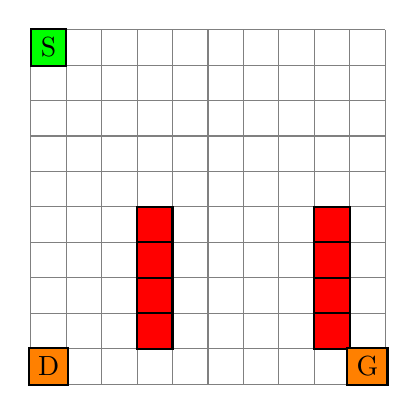
\begin{tikzpicture}[scale=0.45]
\draw[step=1.0 cm,color=gray] (0,0)grid (10,10);
% col, row
\node[rectangle,draw=black,thick, minimum size=0.45cm, fill=green] at (.5,9.5) {S};
\node[rectangle,draw=black,thick, minimum size=0.45cm, fill=red] at (3.5,1.5) {};
%\fill[red!10!white] (0,0) rectangle (1,1);
%\node[fill=green] at (8,8){};  
\node[rectangle,draw=black,thick, minimum size=0.45cm, fill=red] at (3.5,2.5) {};
\node[rectangle,draw=black,thick, minimum size=0.45cm, fill=red] at (3.5,3.5) {};
\node[rectangle,draw=black,thick, minimum size=0.45cm, fill=red] at (3.5,4.5) {};
\node[rectangle,draw=black,thick, minimum size=0.45cm, fill=red] at (8.5,1.5) {};
\node[rectangle,draw=black,thick, minimum size=0.45cm, fill=red] at (8.5,2.5) {};
\node[rectangle,draw=black,thick, minimum size=0.45cm, fill=red] at (8.5,3.5) {};
\node[rectangle,draw=black,thick, minimum size=0.45cm, fill=red] at (8.5,4.5) {};
\node[rectangle,draw=black,thick, minimum size=0.45cm, fill=orange] at (9.5,.5) {G};
\node[rectangle,draw=black,thick, minimum size=0.45cm, fill=orange] at (.5,.5) {D};
\end{tikzpicture}
  		\label{fig:gridworld1}
    }
    &
    \subfigure[2.75\textwidth][Domain-$2$: $10\times 10$ Gridworld] 
    %with $r_{i_{{i}\neq {*}}}=0.07$ and $r^{*}=0.1$
    {
    		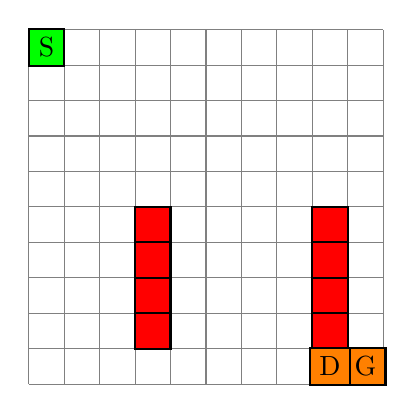
\begin{tikzpicture}[scale=0.45]
\draw[step=1.0 cm,color=gray] (0,0)grid (10,10);
% col, row
\node[rectangle,draw=black,thick, minimum size=0.45cm, fill=green] at (.5,9.5) {S};
\node[rectangle,draw=black,thick, minimum size=0.45cm, fill=red] at (3.5,1.5) {};
\node[rectangle,draw=black,thick, minimum size=0.45cm, fill=red] at (3.5,2.5) {};
\node[rectangle,draw=black,thick, minimum size=0.45cm, fill=red] at (3.5,3.5) {};
\node[rectangle,draw=black,thick, minimum size=0.45cm, fill=red] at (3.5,4.5) {};
\node[rectangle,draw=black,thick, minimum size=0.45cm, fill=red] at (8.5,1.5) {};
\node[rectangle,draw=black,thick, minimum size=0.45cm, fill=red] at (8.5,2.5) {};
\node[rectangle,draw=black,thick, minimum size=0.45cm, fill=red] at (8.5,3.5) {};
\node[rectangle,draw=black,thick, minimum size=0.45cm, fill=red] at (8.5,4.5) {};
\node[rectangle,draw=black,thick, minimum size=0.45cm, fill=orange] at (9.5,.5) {G};
\node[rectangle,draw=black,thick, minimum size=0.45cm, fill=orange] at (8.5,.5) {D};
\end{tikzpicture}
  		\label{fig:gridworld2}
    }
    \end{tabular}
    \end{center}
    \caption{Description of two Toy gridworld domain}
    \label{fig:gridworld}
    \vspace*{-1em}
\end{figure}




\section{Experiments}
\label{review:expt}
\subsection{Toy Gridworld Domain}

In this section, we run Q-learning and Sarsa with linear function approximation in the two gridworld domain shown in Figure \ref{fig:gridworld1} and Figure \ref{fig:gridworld2}. The results of the experiments are shown in Figure \ref{fig:1} and Figure \ref{fig:2} for the domain 1 and 2 respectively. All the algorithms were averaged over $50$ independent trials and each trial consisted of $6000$ episodes.

\textbf{Experiment 1 (Domain 1):} In this experiment we use linear function approximation for both Q-Learning and Sarsa to handle this partially observed environment. From Figure \ref{fig:1} we see that Sarsa performs better than Q-Learning in this Domain and stabilizes before Q-Learning.

\textbf{Experiment 2 (Domain 2):} In this experiment again we use linear function approximation for both Q-Learning and Sarsa to handle this partially observed environment. From Figure \ref{fig:2} we see that Sarsa performs worse than Q-Learning in this Domain. Infact both the algorithms does not stabilize in this experiment. This results from the fact the the entry to the state $S_t = G$ is restricted and both the algorithms spend considerable amount of time in fruitless exploration.


\begin{figure}[!th]
    \begin{center}
    \begin{tabular}{cc}
    \setlength{\tabcolsep}{0.1pt}
    \subfigure[2.75\textwidth][Expt-$1$: $10\times 10$ Gridworld (Domain 1)]
    %with $r_{i_{{i}\neq {*}}}=0.07$ and $r^{*}=0.1$
    {
    		\pgfplotsset{
		tick label style={font=\large},
		label style={font=\large},
		legend style={font=\large},
		ylabel style={yshift=12pt},
		%legend style={legendshift=32pt},
		}
        \begin{tikzpicture}[scale=0.8]
      	\begin{axis}[
		xlabel={Episodes},
		ylabel={Discounted Return},
		grid=major,
        %clip mode=individual,grid,grid style={gray!30},
        clip=true,
        %clip mode=individual,grid,grid style={gray!30},
  		legend style={at={(0.5,1.4)},anchor=north, legend columns=3} ]
      	% UCB
		\addplot table{results/NewExpt/Expt1/comp_subsampled_QlearningA.txt};
		\addplot table{results/NewExpt/Expt1/comp_subsampled_SarsaA.txt};
		\addplot table{results/NewExpt/Expt1/comp_subsampled_QlearningL.txt};
		\addplot table{results/NewExpt/Expt1/comp_subsampled_SarsaL.txt};
      	\legend{Q-Learning, Sarsa, Q($\lambda$), Sarsa($\lambda$)}   
      	\end{axis}
      	\end{tikzpicture}
  		\label{fig:1}
    }
    &
    \subfigure[2.75\textwidth][Expt-$2$: $10\times 10$ Gridworld (Domain 2)] 
    %with $r_{i_{{i}\neq {*}}}=0.07$ and $r^{*}=0.1$
    {
    		\pgfplotsset{
		tick label style={font=\large},
		label style={font=\large},
		legend style={font=\large},
		ylabel style={yshift=12pt},
		%legend style={legendshift=32pt},
		}
        \begin{tikzpicture}[scale=0.8]
      	\begin{axis}[
		xlabel={Episodes},
		ylabel={Discounted Return},
		grid=major,
        %clip mode=individual,grid,grid style={gray!30},
        clip=true,
        %clip mode=individual,grid,grid style={gray!30},
  		legend style={at={(0.5,1.4)},anchor=north, legend columns=3} ]
      	% UCB
		\addplot table{results/NewExpt/Expt2/comp_subsampled_QlearningA.txt};
		\addplot table{results/NewExpt/Expt2/comp_subsampled_SarsaA.txt};
		\addplot table{results/NewExpt/Expt2/comp_subsampled_QlearningL.txt};
		\addplot table{results/NewExpt/Expt2/comp_subsampled_SarsaL.txt};
      	\legend{Q-Learning, Sarsa, Q($\lambda$), Sarsa($\lambda$)}   	
      	\end{axis}
      	\end{tikzpicture}
  		\label{fig:2}
    }
    \end{tabular}
    \end{center}
    \caption{A comparison of the performance of various algorithms. }
    \label{fig:algoExpt}
    \vspace*{-1em}
\end{figure}

\subsection{Classic Domain}

The mountain car was first described in Andrew Moore's Thesis \citep{Efficient memory-based learning for robot control} and was latter properly defined in \citet{DBLP:journals/ml/SinghS96}. The task consist of driving a car resting in a valley up the mountain. The main challenge of this task is that the car by itself cannot drive up the mountain and it has to swing back and forth to gather the sufficient momentum to reach the top of the mountain (see Figure \ref{fig:3}). Nonetheless, this simple environment consist of several challenges that afflicts the medical domain. It's a continuous state space problem, hence function approximation has to be used which makes it a partially observed MDP. Moreover, the car can only accumulate a positive reward of $+50$ when it reaches the top or suffers a negative reward of $-1$ the time while it swings back and forth.  So this models the long horizon problem. The action space is discrete in this toy domain. 

In Figure \ref{fig:4} we show how Q($\lambda$) and Sarsa($\lambda$) along with Fourier basis can be used to solve this problem.

\begin{figure}[!th]
    \begin{center}
    \begin{tabular}{cc}
    \setlength{\tabcolsep}{0.1pt}
    \subfigure[2.75\textwidth][Domain-$3$: Mountain Car]
    %with $r_{i_{{i}\neq {*}}}=0.07$ and $r^{*}=0.1$
    {
    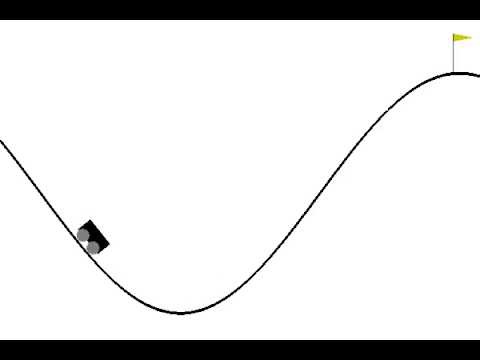
\includegraphics[scale=0.35]{img/mountain_car.jpeg}
    \label{fig:3}
    }
    \setlength{\tabcolsep}{0.1pt}
    \subfigure[2.75\textwidth][Expt-$3$: Mountain Car]
    %with $r_{i_{{i}\neq {*}}}=0.07$ and $r^{*}=0.1$
    {
    		\pgfplotsset{
		tick label style={font=\large},
		label style={font=\large},
		legend style={font=\large},
		ylabel style={yshift=12pt},
		%legend style={legendshift=32pt},
		}
        \begin{tikzpicture}[scale=0.8]
      	\begin{axis}[
		xlabel={Episodes},
		ylabel={Discounted Return},
		grid=major,
        %clip mode=individual,grid,grid style={gray!30},
        clip=true,
        %clip mode=individual,grid,grid style={gray!30},
  		legend style={at={(0.5,1.4)},anchor=north, legend columns=3} ]
      	% UCB
		\addplot table{results/NewExpt/Expt3/comp_subsampled_Qlearning.txt};
		\addplot table{results/NewExpt/Expt3/comp_subsampled_Sarsa.txt};
		\addplot table{results/NewExpt/Expt3/comp_subsampled_Qlearning1.txt};
		\addplot table{results/NewExpt/Expt3/comp_subsampled_Sarsa1.txt};
      	\legend{Q-Learning, Sarsa, Q($\lambda$), Sarsa($\lambda$)}   
      	\end{axis}
      	\end{tikzpicture}
  		\label{fig:4}
    }
    \end{tabular}
    \end{center}
    \caption{A comparison of the performance of various algorithms. }
    \label{fig:algoExpt1}
    \vspace*{-1em}
\end{figure}



\section{Conclusions and Future Works}
\label{review:conc}
In this report we formulated two gadget domains which are easy to handle and yet has sufficient complexities to handle many important and intriguing features of the real-life medical domain. We also showed that both Q-Learning and Sarsa with linear approximation fails to perform well in these domains. Future work includes proposing new algorithm that might perform better in these environments or to test planning algorithms in these domains.

\clearpage
\newpage


\bibliographystyle{apalike}
\bibliography{biblio1}

\end{document}
